\documentclass[a4paper]{article}

\usepackage[english]{babel}
\usepackage{amsmath}
\usepackage{color}
\usepackage{amssymb}
\usepackage{dsfont}
\usepackage{multicol}
%\usepackage[lofdepth,lotdepth]{subfig}  This gives errors when used together with "subcaption", which is needed to create subfigures.
\usepackage{graphicx}
\usepackage{listings}
\usepackage[hyphens]{url}
\usepackage{pgf, tikz}
\usetikzlibrary{arrows, automata}
\usepackage{titling}
\usepackage{varwidth}
\usepackage{hyperref}
\usepackage{color} %red, green, blue, yellow, cyan, magenta, black, white
\definecolor{mygreen}{RGB}{28,172,0} % color values Red, Green, Blue
\definecolor{mylilas}{RGB}{170,55,241}
\setlength\parindent{0pt}
\usepackage{float}
\usepackage{subcaption}
\usepackage{polynom}


\newcommand\independent{\protect\mathpalette{\protect\independenT}{\perp}}
\def\independenT#1#2{\mathrel{\rlap{$#1#2$}\mkern2mu{#1#2}}}

\usepackage{geometry}
 \geometry{
 a4paper,
 total={165mm,257mm},
 left=20mm,
 top=20mm,
 }

\definecolor{codegreen}{rgb}{0,0.6,0}
\definecolor{codegray}{rgb}{0.5,0.5,0.5}
\definecolor{codepurple}{rgb}{0.58,0,0.82}
\definecolor{backcolour}{rgb}{0.95,0.95,0.92}

\lstdefinestyle{mystyle}{
    backgroundcolor=\color{backcolour},   
    commentstyle=\color{codegreen},
    keywordstyle=\color{magenta},
    numberstyle=\tiny\color{codegray},
    stringstyle=\color{codepurple},
    basicstyle=\footnotesize,
    breakatwhitespace=false,         
    breaklines=true,                 
    captionpos=b,                    
    keepspaces=true,                 
    numbers=left,                    
    numbersep=5pt,                  
    showspaces=false,                
    showstringspaces=false,
    showtabs=false,                  
    tabsize=2
}
 
\lstset{style=mystyle}


\title{Statistical Machine Learning 2018\\Assignment 3\\Deadline: 25th of November 2018}
\author{
  Christoph Schmidl\\ s4226887\\      \texttt{c.schmidl@student.ru.nl}
  \and
  Mark Beijer\\ s4354834\\     \texttt{mbeijer@science.ru.nl}
}
\date{\today}

\begin{document}
\maketitle


\section*{Exercise 1 - The faulty lighthouse (weight 5)}

A lighthouse is somewhere off a piece of straight coastline at a position $\alpha$ along the shore and a distance $\beta$ out to sea. Due to a technical fault, as it rotates the light source only occasionally and briefly flickers on and off. As a result it emits short, highly focused beams of light at random intervals. These pulses are intercepted on the coast by photo-detectors that record only the fact that a flash has occurred, but not the angle from which it came. So far, $N$ flashes have been recorded at positions $\mathcal{D} = {x1, . . . , xN }$. Where is the lighthouse?

\begin{figure}[H]
\center
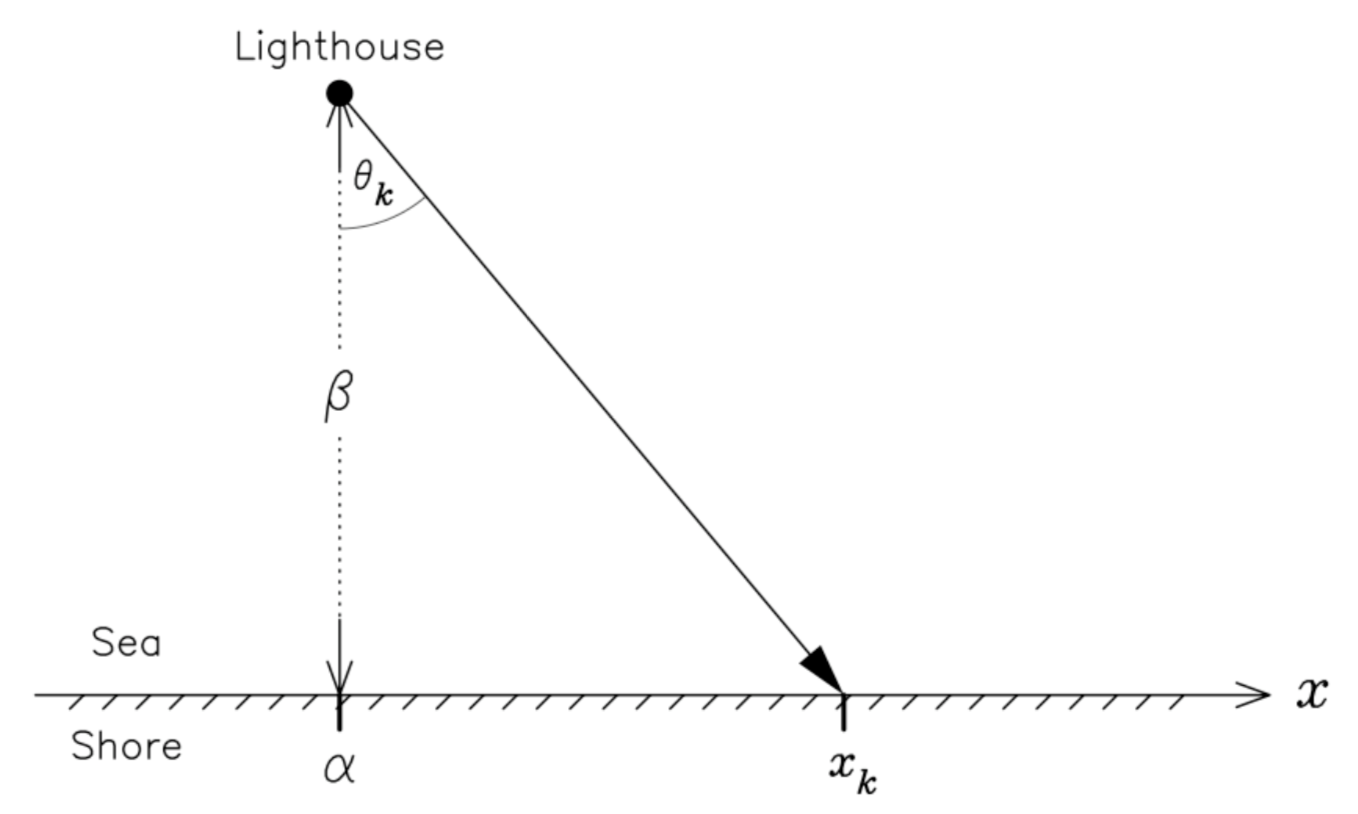
\includegraphics[width=0.75\textwidth]{Images/lighthouse_fig.png}
\caption{Geometry of the lighthouse problem.}
\label{Fig:lighthouse}
\end{figure}




\textbf{Part 1 - Constructing the model}\\

\subsection*{1.1.1}

Let $\theta_k$ be the (unknown) angle for the k-th recorded flash, see fig.1. Argue why

\begin{eqnarray}
p(\theta_k | \alpha, \beta) = \frac{1}{\pi}
\end{eqnarray}

would be a reasonable distribution over $\theta_k$ between $\pm \frac{\pi}{2}$ (zero otherwise).\\


\textbf{Answer:}\\



\subsection*{1.1.2}

We only have the position $x_k$ of the detector that recorded flash $k$, but we can relate this to the unknown $\theta_k$ via elementary geometry as

\begin{eqnarray}
\beta \tan(\theta_k) = x_k - \alpha	
\end{eqnarray}

Show that the expected distribution over $x$ given $\alpha$ and $\beta$ can be written as

\begin{eqnarray}
p(x_k | \alpha, \beta) = \frac{\beta}{\pi [\beta^2 + (x_k - \alpha)^2 ]}
\end{eqnarray}

by using (2) to substitute variable $x_k$ for $\theta_k$ in the distribution (1). Plot the distribution for $\beta = 1$ and a particular value of $\alpha$.\\
Hint: use the Jacobian $|\frac{d \theta}{d x }|$ (Bishop, p.18) and the fact that $(tan^{-1}x)' = \frac{1}{1 + x^2}$.\\



\textbf{Answer:}\\



\subsection*{1.1.3}

Inferring the position of the lighthouse corresponds to estimating $\alpha$ and $\beta$ from the data $\mathcal{D}$. This is still quite difficult, but if we assume that $\beta$ is known, then from Bayes’ theorem we know that $p(\alpha|\mathcal{D}, \beta) \propto p(\mathcal{D}|\alpha, \beta) p(\alpha|\beta)$. We have no a priori knowledge about the position $\alpha$ along the coast other than that it should not depend on the distance out at sea.\\

Show that with these assumptions the log of the posterior density can be written as

\begin{eqnarray}
L = \ln (p(\alpha | \mathcal{D, \beta})) = \texttt{constant} - \sum_{k = 1}^N \ln [\beta^2 + (x_k - \alpha)^2] 
\end{eqnarray}

and give an expression for the value $\hat{\alpha}$ that maximizes this posterior density.\\

\textbf{Answer:}\\


\subsection*{1.1.4}

Suppose we have a data set (in km) of $\mathcal{D} = \{ 3.6, 7.7, -2.6, 4.9, -2.3, 0.2, -7.3, 4.4, 7.3, -5.7\}$. We also assume that the distance $\beta$ from the shore is known to be 2 km. As it is difficult to find a simple expression for the value of $\hat{\alpha}$ that maximizes (4), we try an alternative approach instead.\\

Plot $p(\alpha|\mathcal{D}, \beta = 2)$ as a function of $\alpha$ over the interval $[-10, 10]$. What is your most likely estimate for $\hat{\alpha}$ based on this graph? Compare with the mean estimate of the dataset. Can you explain the difference?\\


\textbf{Answer:}\\




\end{document}
